% Quantitative research portfolio report: cross-validated equity derivatives on SPX.
% Build: pdflatex portfolio_report && bibtex portfolio_report && pdflatex portfolio_report && pdflatex portfolio_report
\documentclass[10pt,letterpaper]{article}

% ---------------------------------------------------------------- fonts and layout
\usepackage[T1]{fontenc}
\usepackage{lmodern}
\usepackage[scaled=0.95]{helvet}
\renewcommand{\familydefault}{\sfdefault}
\usepackage{amsmath,amssymb,bm}
\usepackage[letterpaper,top=0.95in,bottom=0.9in,left=0.85in,right=0.85in,headsep=0.35in]{geometry}
\usepackage[letterspace=180]{microtype}
\usepackage{graphicx,xcolor,booktabs,array,tabularx,enumitem,ragged2e}
\usepackage{tikz}
\usepackage[most]{tcolorbox}
\usepackage{titlesec,fancyhdr,caption,float}
\usepackage[section]{placeins}
\usepackage{needspace}
\usepackage[authoryear,round]{natbib}
\usepackage[hidelinks]{hyperref}
\graphicspath{{../figures/}}

\setlength{\parindent}{0pt}
\setlength{\parskip}{6pt}
\linespread{1.08}

% ---------------------------------------------------------------- palette
\definecolor{navy}{HTML}{0A1728}
\definecolor{ink}{HTML}{102A43}
\definecolor{accent}{HTML}{2F6BFF}
\definecolor{teal}{HTML}{00A896}
\definecolor{tealbright}{HTML}{3DD6BC}
\definecolor{muted}{HTML}{7A8699}
\definecolor{captxt}{HTML}{50607A}
\definecolor{tilecover}{HTML}{3C4654}
\definecolor{bluebg}{HTML}{EAF1FF}
\definecolor{redbg}{HTML}{FFF0F0}
\definecolor{redbar}{HTML}{EF6A6A}
\definecolor{tealbg}{HTML}{E9F8F5}
\definecolor{greybg}{HTML}{F6F8FC}
\definecolor{rulegrey}{HTML}{D8DDE4}
\hypersetup{colorlinks=true,linkcolor=accent,citecolor=teal,urlcolor=teal,
  pdftitle={From Three Prices to One Hedge: Equity Derivatives on SPX},pdfauthor={Kexin (Eve) Zhang}}

% ---------------------------------------------------------------- headings
\titleformat{\section}{\normalfont\fontsize{17}{20}\bfseries\color{navy}}
  {\textcolor{accent}{\thesection}}{0.6em}{}[\vspace{2pt}{\color{rulegrey}\titlerule[0.6pt]}]
\titleformat{\subsection}{\normalfont\large\bfseries\color{navy}}{\thesubsection}{0.6em}{}
\titleformat{\subsubsection}{\normalfont\normalsize\bfseries\color{navy}}{\thesubsubsection}{0.6em}{}
\titlespacing*{\section}{0pt}{16pt}{8pt}
\titlespacing*{\subsection}{0pt}{12pt}{4pt}
\titlespacing*{\subsubsection}{0pt}{8pt}{2pt}

% spaced small-caps style label, as used for "THE RESEARCH QUESTION"
\newcommand{\kicker}[2][accent]{{\color{#1}\footnotesize\bfseries\textls{\MakeUppercase{#2}}}}

% ---------------------------------------------------------------- header and footer
\pagestyle{fancy}
\fancyhf{}
\renewcommand{\headrulewidth}{0pt}
\renewcommand{\sectionmark}[1]{\markboth{\thesection\quad #1}{}}
\fancyhead[L]{\color{muted}\scriptsize\bfseries\textls{KEXIN ZHANG / QUANT RESEARCH}}
\fancyhead[R]{\color{muted}\scriptsize\leftmark}
\fancyfoot[L]{\color{muted}\scriptsize Independent research portfolio}
\fancyfoot[R]{\color{accent}\small\bfseries\thepage}

% ---------------------------------------------------------------- captions
\captionsetup{font={small,color=captxt},labelfont={bf,color=navy},labelsep=colon,
  justification=justified,singlelinecheck=false}
\captionsetup[table]{position=top,skip=6pt}

% ---------------------------------------------------------------- boxes
\newtcolorbox{callout}[1][accent]{enhanced,colback=bluebg,colframe=bluebg,
  borderline west={3pt}{0pt}{#1},sharp corners,boxrule=0pt,left=10pt,right=10pt,top=7pt,bottom=7pt,
  before skip=10pt,after skip=10pt}
\newtcolorbox{caution}{enhanced,colback=redbg,colframe=redbg,
  borderline west={3pt}{0pt}{redbar},sharp corners,boxrule=0pt,left=10pt,right=10pt,top=7pt,bottom=7pt,
  before skip=10pt,after skip=10pt}
\newtcolorbox{darkbox}{enhanced,colback=ink,colframe=ink,arc=4pt,boxrule=0pt,
  left=12pt,right=12pt,top=9pt,bottom=9pt,fontupper=\color{white}}
% stat tile: #1 background, #2 number, #3 label
\newcommand{\stattile}[3]{%
  \begin{tcolorbox}[enhanced,colback=#1,colframe=#1,arc=4pt,boxrule=0pt,left=9pt,right=6pt,top=8pt,bottom=8pt,
    width=\linewidth,height=1.25in,valign=center]
  {\fontsize{19}{22}\selectfont\bfseries\color{navy}#2}\\[5pt]
  \parbox{\linewidth}{\raggedright\hyphenpenalty=10000\color{captxt}\tiny\bfseries\textls{\MakeUppercase{#3}}}
  \end{tcolorbox}}

\setlist[itemize]{label={\color{navy}\textbullet},leftmargin=1.3em,itemsep=3pt,topsep=2pt,parsep=0pt}
\setlist[enumerate]{leftmargin=1.6em,itemsep=3pt,topsep=2pt,parsep=0pt}

\newcommand{\vp}{\,vol pt}
\renewcommand{\arraystretch}{1.18}

\begin{document}

% ================================================================= COVER
\thispagestyle{empty}
\begin{tikzpicture}[remember picture,overlay]
  \fill[navy] (current page.south west) rectangle (current page.north east);
  \fill[accent] (current page.north west) rectangle ([yshift=-0.12in]current page.north east);
  \draw[white,opacity=0.08,line width=0.8pt] ([xshift=-1.0in,yshift=3.3in]current page.south east) circle (3.3in);
  \draw[white,opacity=0.06,line width=0.8pt] ([xshift=-0.2in,yshift=1.3in]current page.south east) circle (2.4in);
  % thin stylised smile in the background
  \draw[tealbright,opacity=0.18,line width=1.1pt]
    plot[smooth] coordinates {([xshift=-4.6in,yshift=5.2in]current page.south east)
      ([xshift=-3.6in,yshift=4.45in]current page.south east) ([xshift=-2.6in,yshift=3.95in]current page.south east)
      ([xshift=-1.8in,yshift=3.85in]current page.south east) ([xshift=-1.1in,yshift=4.05in]current page.south east)};
\end{tikzpicture}

\vspace*{0.15in}
{\color{teal}\rule{0.25in}{5pt}}\par\vspace{2pt}
\kicker[tealbright]{Quantitative Research Portfolio}

\vspace{0.55in}
{\color{white}\fontsize{31}{40}\selectfont\bfseries From Three Prices\\ to One Hedge:\\ Equity Derivatives on SPX\par}

\vspace{0.18in}
{\color{white}\large Three-Way Pricing Cross-Validation $\rightarrow$ SPX Calibration\\[4pt]
Exotic Model Risk $\rightarrow$ Hedging-Error Attribution\par}

\vspace{0.3in}
{\color{teal}\rule{1.25in}{1.2pt}}

\vspace{0.25in}
\begin{minipage}{0.82\textwidth}
{\color{white}\bfseries Fourier, PDE and Monte Carlo engines agree on every price; real SPX quotes then
decide how much the choice of model matters for calibration, for an autocallable, and for the hedge.\par}
\end{minipage}

\vfill
\newcommand{\covertile}[2]{%
  \begin{tcolorbox}[enhanced,colback=tilecover,colframe=tilecover,arc=4pt,boxrule=0pt,left=10pt,top=9pt,bottom=9pt,width=\linewidth]
  {\color{white}\fontsize{19}{22}\selectfont\bfseries #1}\\[4pt]{\color{white}\tiny\bfseries\textls{\MakeUppercase{#2}}}
  \end{tcolorbox}}
\begin{minipage}[t]{0.31\textwidth}\covertile{2.00}{Crank--Nicolson order}\end{minipage}\hfill
\begin{minipage}[t]{0.31\textwidth}\covertile{\textcolor{tealbright}{14.0--16.0\%}}{Autocall coupon across models}\end{minipage}\hfill
\begin{minipage}[t]{0.31\textwidth}\covertile{91\%}{Hedged P\&L variance explained}\end{minipage}

\vspace{0.3in}
{\color{white}\bfseries Kexin (Eve) Zhang\par}
\vspace{4pt}
{\color{white}\small Independent Research Project \quad/\quad October 2026\par}
\vspace{3pt}
{\color{teal}\small kexinzhang0209@gmail.com\par}

\vspace{0.25in}
{\color{white}\tiny SPX end-of-day option quotes (optionsDX) \ \textbullet\ \ 4.93 million quotes \ \textbullet\ \ 311 quote dates \ \textbullet\ \ Jan--Mar 2020 and Jan--Dec 2023\par
\vspace{3pt}
Coupon range: Black-Scholes, Heston and Dupire local vol, all fitted to the 2023-01-18 surface. P\&L explained: daily variance, 2020 Q1 and 2023.\par
\vspace{3pt}
Independent research demonstration. Not investment advice.\par}
\vspace*{0.05in}
\newpage

% ================================================================= EXECUTIVE SNAPSHOT
\pagenumbering{arabic}
\markboth{Executive Snapshot}{}
\section*{Executive Snapshot}

\kicker{The research question}
\vspace{-2pt}
\begin{callout}
\large\bfseries\color{navy}
Do three independent numerical methods produce the same price, and once a model is fitted to real
SPX options, how much do its remaining degrees of freedom move exotic prices and hedging P\&L?
\end{callout}

\kicker{Evidence in four numbers}\par\vspace{2pt}
\begin{minipage}[t]{0.235\textwidth}\stattile{bluebg}{2.00}{PDE convergence order}\end{minipage}\hfill
\begin{minipage}[t]{0.235\textwidth}\stattile{redbg}{0.89\,vol pt}{Heston SPX fit RMSE}\end{minipage}\hfill
\begin{minipage}[t]{0.235\textwidth}\stattile{tealbg}{+2.0\,pts}{Autocall coupon, BS to LV}\end{minipage}\hfill
\begin{minipage}[t]{0.235\textwidth}\stattile{greybg}{91\%}{P\&L variance explained}\end{minipage}

\vspace{8pt}
\begin{minipage}[t]{0.48\textwidth}
\kicker{What the evidence says}
\begin{itemize}
\item Closed form, COS, Crank--Nicolson and Monte Carlo agree on a Black-Scholes call to four
decimals (12.0056); Heston COS and QE Monte Carlo agree within 0.2 standard errors.
\item Convergence rates are measured, not assumed: PDE slope $-2.00$, exponential COS
convergence, Monte Carlo error $\propto n^{-1/2}$ with an 8$\times$ variance cut from a control variate.
\item On the SPX surface the Heston calibration is stable in $\rho$ (CV 3\%), but $\kappa$ and $\xi$
move together (weekly-change correlation 0.96): the ridge predicted beforehand on synthetic data.
\item Three models fitted to the same surface give a 3-year autocallable a fair coupon of
14.0\%, 15.2\% and 16.0\%.
\end{itemize}
\end{minipage}\hfill
\begin{minipage}[t]{0.48\textwidth}
\kicker{What requires caution}
\begin{itemize}
\item Heston misses the 1-month skew (1.48\vp{} error); no single diffusive model fits
the whole surface inside the bid--ask spread.
\item The real hedging backtest covers 15 monthly trades over two windows. It shows the
\emph{source} of P\&L, not a statistically reliable strategy return.
\item The March 2020 trade is truncated at the data cut-off, so the 2020 Q1 loss is a lower bound.
\item No 2D Heston PDE and no stochastic local vol yet; quotes are end-of-day mids from one vendor.
\end{itemize}
\end{minipage}

\vspace{10pt}
\begin{darkbox}
\kicker[tealbright]{What the project demonstrates}\par\vspace{2pt}
{\large\bfseries A pricing library whose every number is checked by a second, independent method.}\par\vspace{2pt}
{\small That discipline is what makes the later claims believable: when Heston and local vol disagree on
an autocallable by 0.8 coupon points, the gap is model risk, not numerical error.}
\end{darkbox}

\vfill
{\color{muted}\scriptsize Data: SPX end-of-day quotes, optionsDX, Jan--Mar 2020 and Jan--Dec 2023. Showcase date 2023-01-18 (spot 3945.1).
All engines and tests run on synthetic inputs; 70 unit tests run in continuous integration.}
\newpage

% ================================================================= 1 ARCHITECTURE
\section{Research Architecture}
\subsection{Research sequence}
The project is built in four stages, each of which reuses only what the previous stage has already
validated. A pricing error in stage 1 would contaminate every later number, so the order is deliberate:
numerics first, market data second, products third, risk last.

\subsubsection{Questions}
\begin{enumerate}
\item \textbf{Numerics:} do Fourier, finite-difference and simulation methods give the same price for the
same contract, and does each converge at its theoretical rate \citep{fang2008,andersen2008,longstaff2001}?
\item \textbf{Calibration:} how well do Heston \citep{heston1993}, SABR \citep{hagan2002} and Dupire local vol
\citep{dupire1994} fit the SPX surface, and which parameters are actually identified by it?
\item \textbf{Model risk:} if three models reproduce the same vanilla market, how far apart are their prices for
path-dependent products (a barrier put and an autocallable)?
\item \textbf{Hedging:} where does the P\&L of a delta-hedged option come from, and how much of it can the
Greeks explain on real data?
\end{enumerate}

Each stage has a validation step that does not depend on the market: a closed form, a limiting case, or a
synthetic surface whose true parameters are known. Real data enter only after the method has passed on
synthetic data. That separation is what allows a fit error on SPX to be read as model error rather
than as a bug.

\subsection{Data and cleaning}
End-of-day SPX option quotes (16:00 ET) were taken from optionsDX for January--March 2020 (the COVID crash)
and all of 2023 (a calm, rising market). Each row carries bid and ask for the call and the put at one
strike and expiry, together with the index level. A single loader maps optionsDX, OptionMetrics and
Yahoo snapshots to one schema, so the cleaning and calibration code never sees vendor formats.

Filters, applied per quote date and expiry:
\begin{itemize}
\item two-sided quotes only: positive bid, ask above bid, mid of at least 0.05;
\item relative spread $(\text{ask}-\text{bid})/\text{mid} \le 50\%$, and at least 7 days to expiry;
\item standardised log-moneyness $\ln(K/F)/(0.2\sqrt{T})$ between $-4$ and $2.5$, where SPX quotes are liquid;
\item out-of-the-money options only: puts below the forward, calls above it.
\end{itemize}

The forward and discount factor are not assumed. For every strike quoted on both sides, put--call parity
gives
\begin{equation}
C(K) - P(K) = D\,(F - K),
\end{equation}
which is linear in $K$. A regression on near-the-money strikes gives the slope $-D$ and intercept $DF$.
No stale spot, assumed dividend yield or external rate curve enters the surface.

\begin{table}[H]
\caption{Data and audit summary}
\begin{tabularx}{\textwidth}{Xr}
\toprule
\textbf{Item} & \textbf{Value}\\
\midrule
Raw option quotes (calls and puts) & 4,930,870\\
Quote dates & 311\\
Distinct expiries & 378\\
Two-sided share of raw quotes & 94.7\%\\
Duplicate date--expiry--strike--type rows & 0\\
Showcase date 2023-01-18: raw quotes $\rightarrow$ cleaned OTM surface & 15,106 $\rightarrow$ 5,498 (44 expiries)\\
Calibration subset (8 tenors, 1 month to 2 years, 25 strikes each) & 197\\
Weekly calibrations (2020 Q1 / 2023) & 14 / 59\\
\bottomrule
\end{tabularx}
\end{table}

\subsection{Models and notation}
Under the risk-neutral measure with rate $r$ and dividend yield $q$, the Heston model is
\begin{equation}
\frac{dS_t}{S_t} = (r-q)\,dt + \sqrt{v_t}\,dW^S_t,\qquad
dv_t = \kappa(\theta - v_t)\,dt + \xi\sqrt{v_t}\,dW^v_t,\qquad d\langle W^S,W^v\rangle_t = \rho\,dt .
\end{equation}
Its characteristic function is known in closed form; the code uses the ``little Heston trap''
formulation \citep{albrecher2007}, which avoids the branch-cut discontinuity of the complex logarithm
at long maturities. The COS method \citep{fang2008} expands the density of $x=\ln(S_T/K)$ in a cosine
series on a truncation interval $[a,b]$:
\begin{equation}
V_0 \approx e^{-rT}\sideset{}{'}\sum_{k=0}^{N-1}\operatorname{Re}\!\left[\varphi\!\left(\frac{k\pi}{b-a}\right)
e^{-ik\pi\frac{a}{b-a}}\right] V_k ,
\end{equation}
where $\varphi$ is the characteristic function, $V_k$ are the cosine coefficients of the payoff (closed form for
calls and puts), and the prime halves the first term. The interval comes from the cumulants of $x$, which
are computed numerically from the cumulant generating function.

Local volatility is obtained from total implied variance $w(y,T)=\sigma_{\text{imp}}^2T$ at
log-moneyness $y=\ln(K/F)$ \citep{gatheral2006}:
\begin{equation}
\sigma_{\text{loc}}^2(y,T) = \frac{\partial_T w}{1 - \frac{y}{w}\partial_y w
+ \frac14\left(-\frac14 - \frac1w + \frac{y^2}{w^2}\right)(\partial_y w)^2 + \frac12\partial_{yy} w}.
\end{equation}
Each expiry is first fitted with an SVI slice \citep{gatheral2014}, so the derivatives in the formula are
analytic in $y$; the $T$-derivative uses linear interpolation in total variance between slices.

\subsection{Validation protocol}
Every reported number has an independent check:
\begin{itemize}
\item \textbf{Prices:} a second engine of a different type (Fourier vs PDE vs simulation), and a third where possible.
\item \textbf{Monte Carlo:} agreement is judged in standard errors, never in decimals.
\item \textbf{Convergence:} log--log slopes against the grid size or path count, compared with theory.
\item \textbf{Calibration:} parameter recovery on synthetic surfaces, with and without added quote noise, before any SPX fit.
\item \textbf{Hedging:} the simulated hedging error is compared with the Kamal--Derman formula before attributing real P\&L.
\end{itemize}

% ================================================================= 2 ENGINES
\section{Three Engines, One Price}
\subsection{Cross-validation table}
Table~\ref{tab:xval} prices three contracts with every applicable engine. Black-Scholes and Heston
use $S=100$, $K=95$, $T=0.75$, $r=4\%$, $q=1.5\%$; the Heston parameters are those of
\citet{fang2008} ($v_0=0.0175$, $\kappa=1.58$, $\theta=0.0398$, $\xi=0.575$, $\rho=-0.571$), which
violate the Feller condition, so the variance process touches zero. This is the hard case for
simulation, handled by the Andersen quadratic-exponential scheme \citep{andersen2008}.

\begin{table}[H]
\caption{Cross-validation of pricing engines}\label{tab:xval}
\centering
\begin{tabular}{lrrrr}
\toprule
\textbf{Product} & \textbf{Closed form} & \textbf{COS} & \textbf{Crank--Nicolson} & \textbf{Monte Carlo ($\pm$1 s.e.)}\\
\midrule
European call, Black-Scholes & 12.0056 & 12.0056 & 12.0057 & 12.0042 $\pm$ 0.0058\\
European call, Heston & -- & 5.7852 & -- & 5.7838 $\pm$ 0.0071\\
American put ($S=36$, $K=40$) & -- & -- & 4.4867 & 4.4758 $\pm$ 0.0065\\
\bottomrule
\end{tabular}
\end{table}

The American put uses the \citet{longstaff2001} test case. The PDE handles early exercise with a penalty
method; Longstaff--Schwartz uses a Laguerre basis on 50 exercise dates, with the exercise rule fitted on one
set of paths and applied to another. An out-of-sample rule is sub-optimal by construction, so its value is a
\emph{lower} bound for the 50-date Bermudan, which is itself below the American. The PDE value sits above the
Monte Carlo value, as it should.

\begin{callout}
\textbf{Published benchmarks have errors too.} The finite-difference value 4.478 quoted for this American
put in \citet{longstaff2001} is off by 0.009. A 20,000-step binomial tree confirms 4.4867, the
Crank--Nicolson value. Without a second engine this discrepancy would have looked like a bug in the PDE.
\end{callout}

\subsection{Convergence rates}
Crank--Nicolson is second order in both space and time, but only if the payoff kink does not pollute the
solution. Two details matter. First, the payoff is averaged over the grid cell that contains the strike.
Second, the first steps use fully implicit half-steps (Rannacher start-up, \citealp{rannacher1984}). The
Crank--Nicolson amplification factor tends to $-1$ for stiff modes, so the high-frequency error created by the
kink is never damped; implicit steps damp it immediately.

\begin{figure}[htbp]
\centering
\begin{minipage}{0.49\textwidth}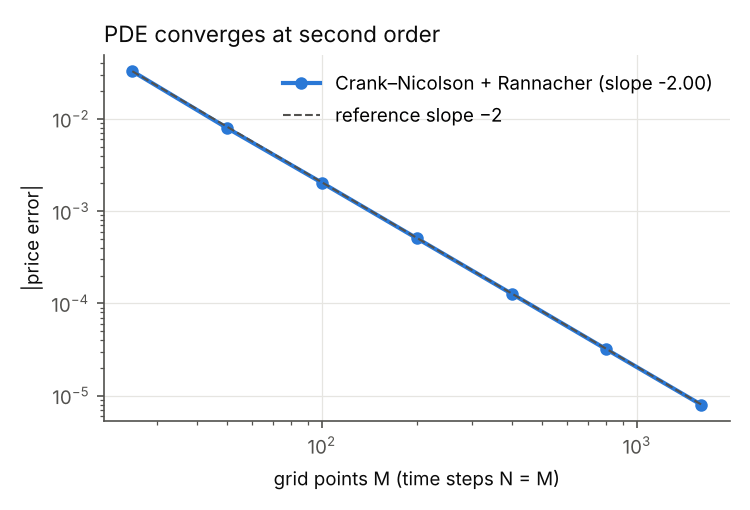
\includegraphics[width=\linewidth]{pde_convergence.png}\end{minipage}\hfill
\begin{minipage}{0.49\textwidth}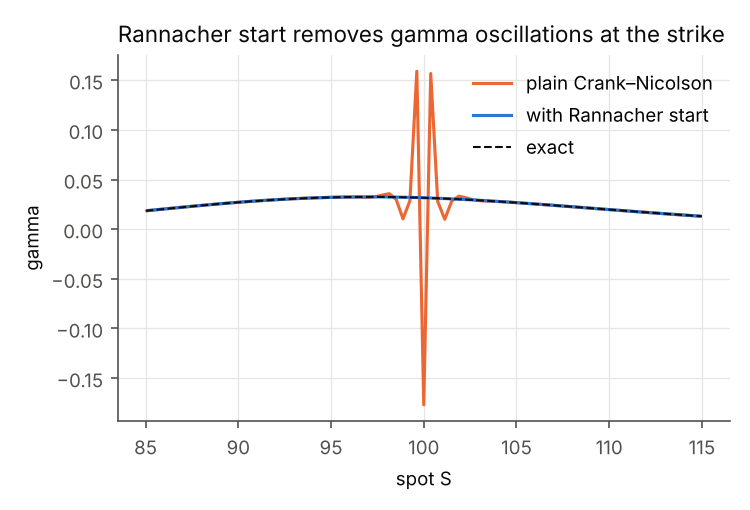
\includegraphics[width=\linewidth]{rannacher_gamma.png}\end{minipage}
\caption{Left: the Crank--Nicolson price error falls with slope $-2.00$ when space and time are refined
together. Right: with 25 time steps, plain Crank--Nicolson leaves a gamma spike of about 0.2 at the strike;
four implicit half-steps remove it (error $10^{-5}$).}
\end{figure}

\begin{figure}[htbp]
\centering
\begin{minipage}{0.49\textwidth}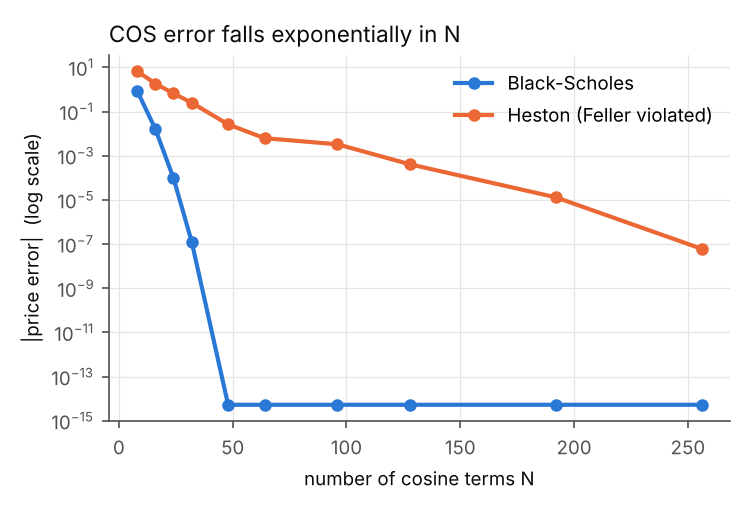
\includegraphics[width=\linewidth]{cos_convergence.png}\end{minipage}\hfill
\begin{minipage}{0.49\textwidth}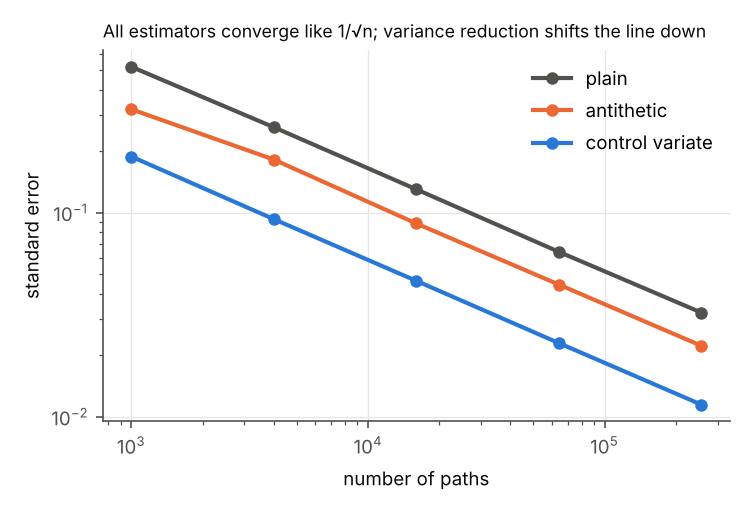
\includegraphics[width=\linewidth]{mc_variance_reduction.png}\end{minipage}
\caption{Left: COS converges exponentially in the number of terms; Black-Scholes reaches machine precision by
$N\approx 64$, Heston with the Feller condition violated needs more terms because its density is less smooth.
Right: all Monte Carlo estimators converge as $n^{-1/2}$; antithetic sampling cuts the variance 2.1$\times$ and the
control variate $e^{-rT}S_T$ cuts it 8.0$\times$.}
\end{figure}

Two further numerical lessons came from the exotics. A knock-out barrier that falls between grid nodes
reduces the PDE to first order; aligning the grid so that the barrier is exactly a node restores second
order. For the autocallable, the value jumps at the autocall level and at the knock-in barrier; giving the
node on each discontinuity the average of its two one-sided values turns first-order convergence into
near-exact agreement with Monte Carlo by 300 space nodes.

% ================================================================= 3 CALIBRATION
\section{Calibrating to the SPX Surface}
\subsection{Objective}
The calibration minimises vega-weighted price errors over the 197 options in the calibration subset:
\begin{equation}
\min_{\Theta}\ \sum_i \left(\frac{C^{\text{model}}_i(\Theta) - C^{\text{mkt}}_i}{\max(\mathcal{V}_i,\ \underline{\mathcal{V}})}\right)^2,
\end{equation}
where $\mathcal{V}_i$ is the Black-Scholes vega and the floor $\underline{\mathcal{V}}$ is 1\% of the median
vega. To first order each term is an implied-vol error, so the objective is measured in vol points while
avoiding a root-finding step inside the optimiser. A bounded trust-region least-squares solver runs from
several starting points; on the showcase date four of four starts reach the same minimum.

Before the SPX fit, the calibrator was run on synthetic Heston surfaces. It recovers the true parameters to
$10^{-4}$, and with 0.2 vol points of quote noise added the fit stops at the noise level (RMSE 0.16\vp).

\subsection{One date in detail: 2023-01-18}
\begin{figure}[htbp]
\centering
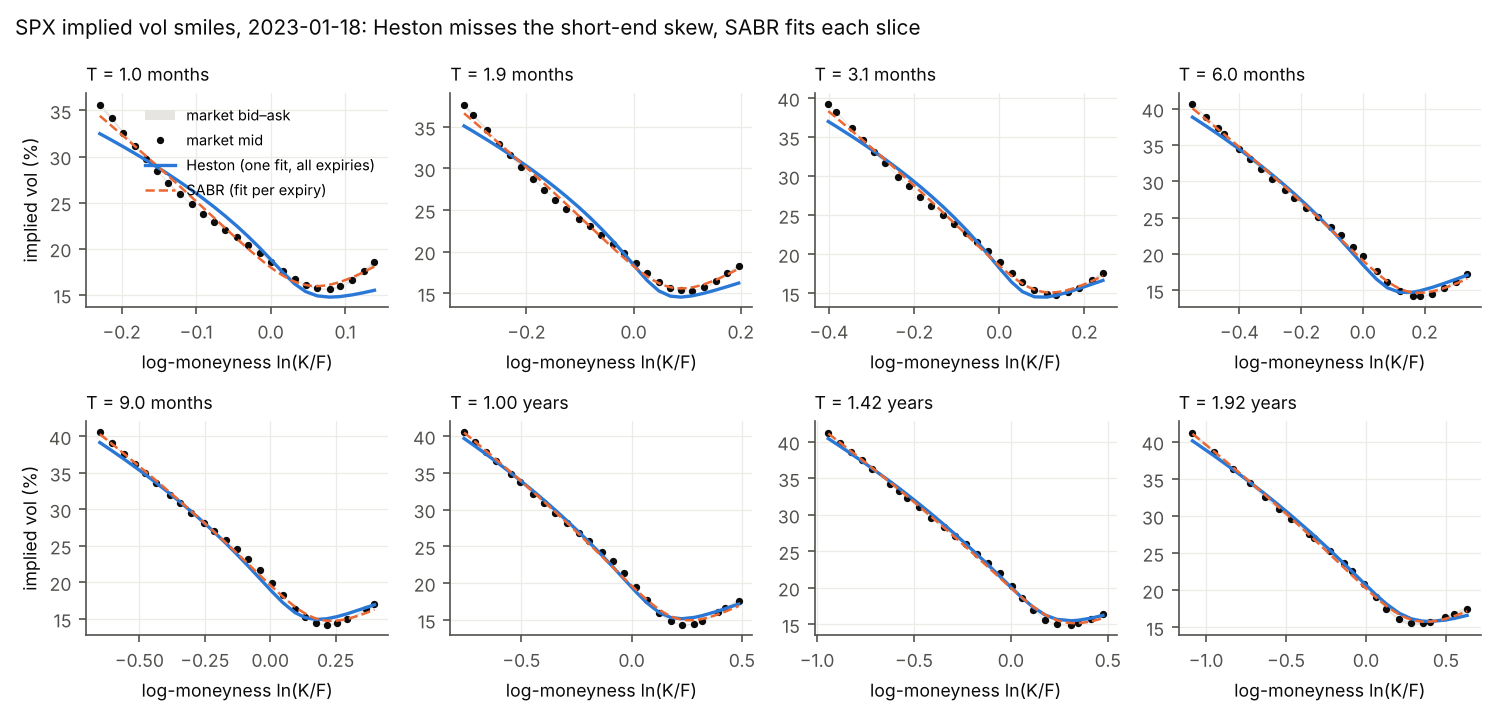
\includegraphics[width=\textwidth]{spx_smiles_fit.png}
\caption{SPX implied vol smiles on 2023-01-18 with the market bid--ask band. One Heston parameter set
(all expiries) misses the short-dated skew; SABR, refitted on every expiry, follows each slice.}
\end{figure}

\begin{table}[H]
\caption{Fit quality on 2023-01-18 (implied-vol RMSE)}
\centering
\begin{tabular}{lrr}
\toprule
\textbf{Expiry set} & \textbf{Heston (5 parameters, whole surface)} & \textbf{SABR (3 per expiry, $\beta=1$)}\\
\midrule
All expiries & 0.89\vp & 0.43\vp\\
1 month & 1.48\vp & 0.54\vp\\
2 years & 0.49\vp & 0.35\vp\\
\bottomrule
\end{tabular}
\end{table}

The fitted Heston parameters are $v_0=0.039$, $\kappa=1.89$, $\theta=0.072$, $\xi=0.97$, $\rho=-0.71$, with
Feller ratio $2\kappa\theta/\xi^2 = 0.29$. The Feller condition is violated, which is typical for equity index
surfaces: the steep skew requires a vol of vol that the condition does not allow.

\begin{figure}[htbp]
\centering
\begin{minipage}{0.48\textwidth}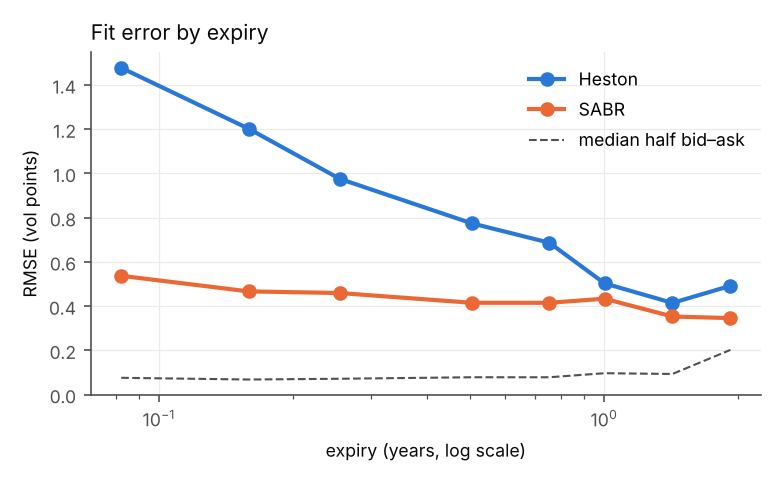
\includegraphics[width=\linewidth]{spx_fit_error_by_expiry.png}\end{minipage}\hfill
\begin{minipage}{0.50\textwidth}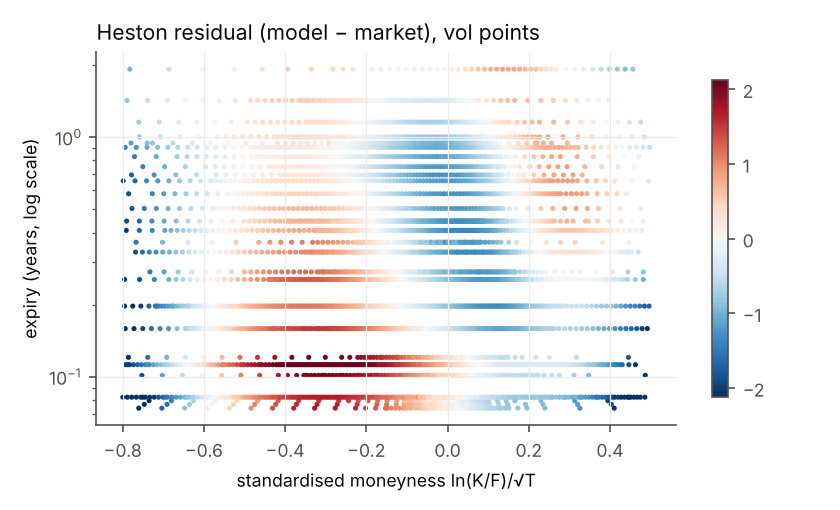
\includegraphics[width=\linewidth]{spx_heston_residuals.png}\end{minipage}
\caption{Left: Heston's fit error falls steadily with maturity; SABR's is flat. Both stay above the median half
bid--ask spread. Right: Heston residuals are structured. At short maturities the model is too low in the deep
put wing and too high around the money.}
\end{figure}

\begin{callout}
\textbf{A model error, not a fitting failure.} In Heston the short-dated skew comes only from the correlated
variance diffusion, which needs time to act. The market's 1-month skew is steeper than a diffusive
stochastic-vol model can produce without extreme vol of vol. That is the standard motivation for jumps (Bates)
or rough volatility, and the residual map shows exactly that signature.
\end{callout}

SABR's per-expiry fit is better for a different reason. Its vol of vol $\nu$ decays from 2.25 at one
month to 0.58 at two years, roughly as $T^{-0.45}$. The term structure is absorbed into parameters that
change with maturity, so SABR is an interpolator of each slice rather than a dynamic model of the surface.

\subsection{Local volatility}
Dupire local vol built from the SVI slices reproduces the vanilla surface by construction (verified on
synthetic data to 0.03\vp). Its at-the-money skew is 1.95 times the implied skew, close to the
short-maturity rule that implied vol at strike $K$ is roughly the average of local vol between spot and $K$,
so the implied slope is half the local slope.

\begin{figure}[htbp]
\centering
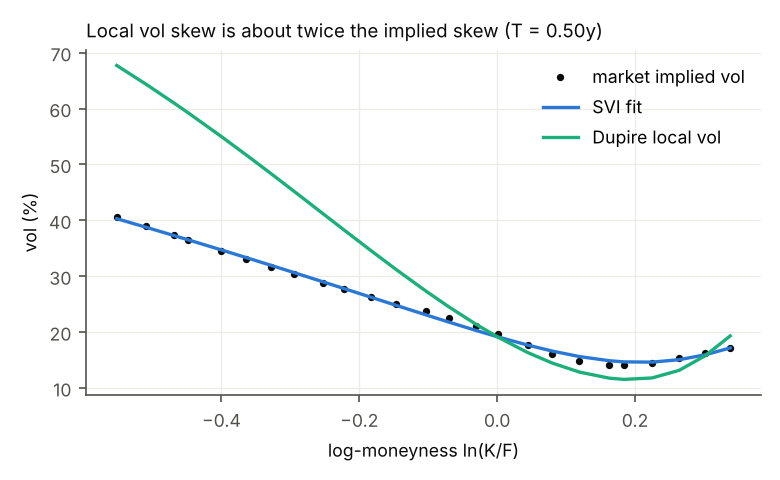
\includegraphics[width=0.62\textwidth]{spx_local_vs_implied.png}
\caption{Market implied vol, SVI fit and Dupire local vol at $T=0.5$ years on 2023-01-18. The local-vol skew is
about twice the implied skew.}
\end{figure}

% ================================================================= 4 STABILITY
\section{Parameter Stability and Identifiability}
\subsection{What the surface actually identifies}
A good fit on one date says nothing about whether the parameters mean anything. The project therefore
asked the identifiability question twice: first on synthetic data, where the answer is known, and then on 73
weekly SPX calibrations.

On synthetic surfaces a $\kappa$ profile (fix $\kappa$, recalibrate the other four parameters) is flat around
the true value when the surface contains only short expiries: $\xi$ moves to compensate, and the fit barely
changes. The prediction was therefore that on real data $\kappa$ and $\xi$ would not be separately pinned down.

\begin{figure}[htbp]
\centering
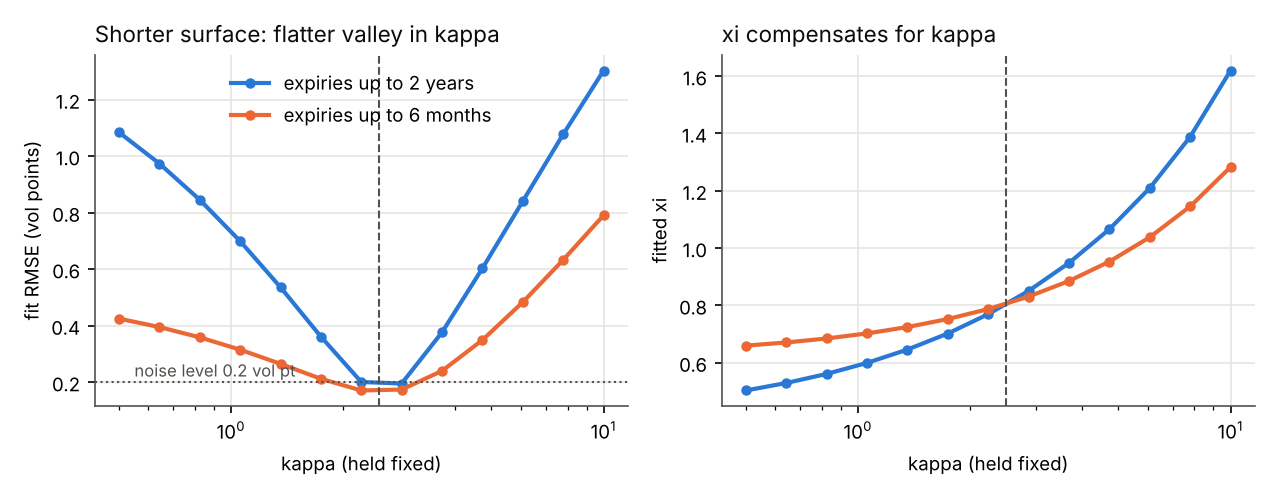
\includegraphics[width=0.85\textwidth]{heston_kappa_profile.png}
\caption{Synthetic Heston surface. Left: the fit RMSE as a function of a fixed $\kappa$ has a flat valley, flatter
when only expiries up to 6 months are used. Right: the fitted $\xi$ rises with $\kappa$ along the valley.}
\end{figure}

\subsection{Weekly SPX calibrations}
\begin{figure}[H]
\centering
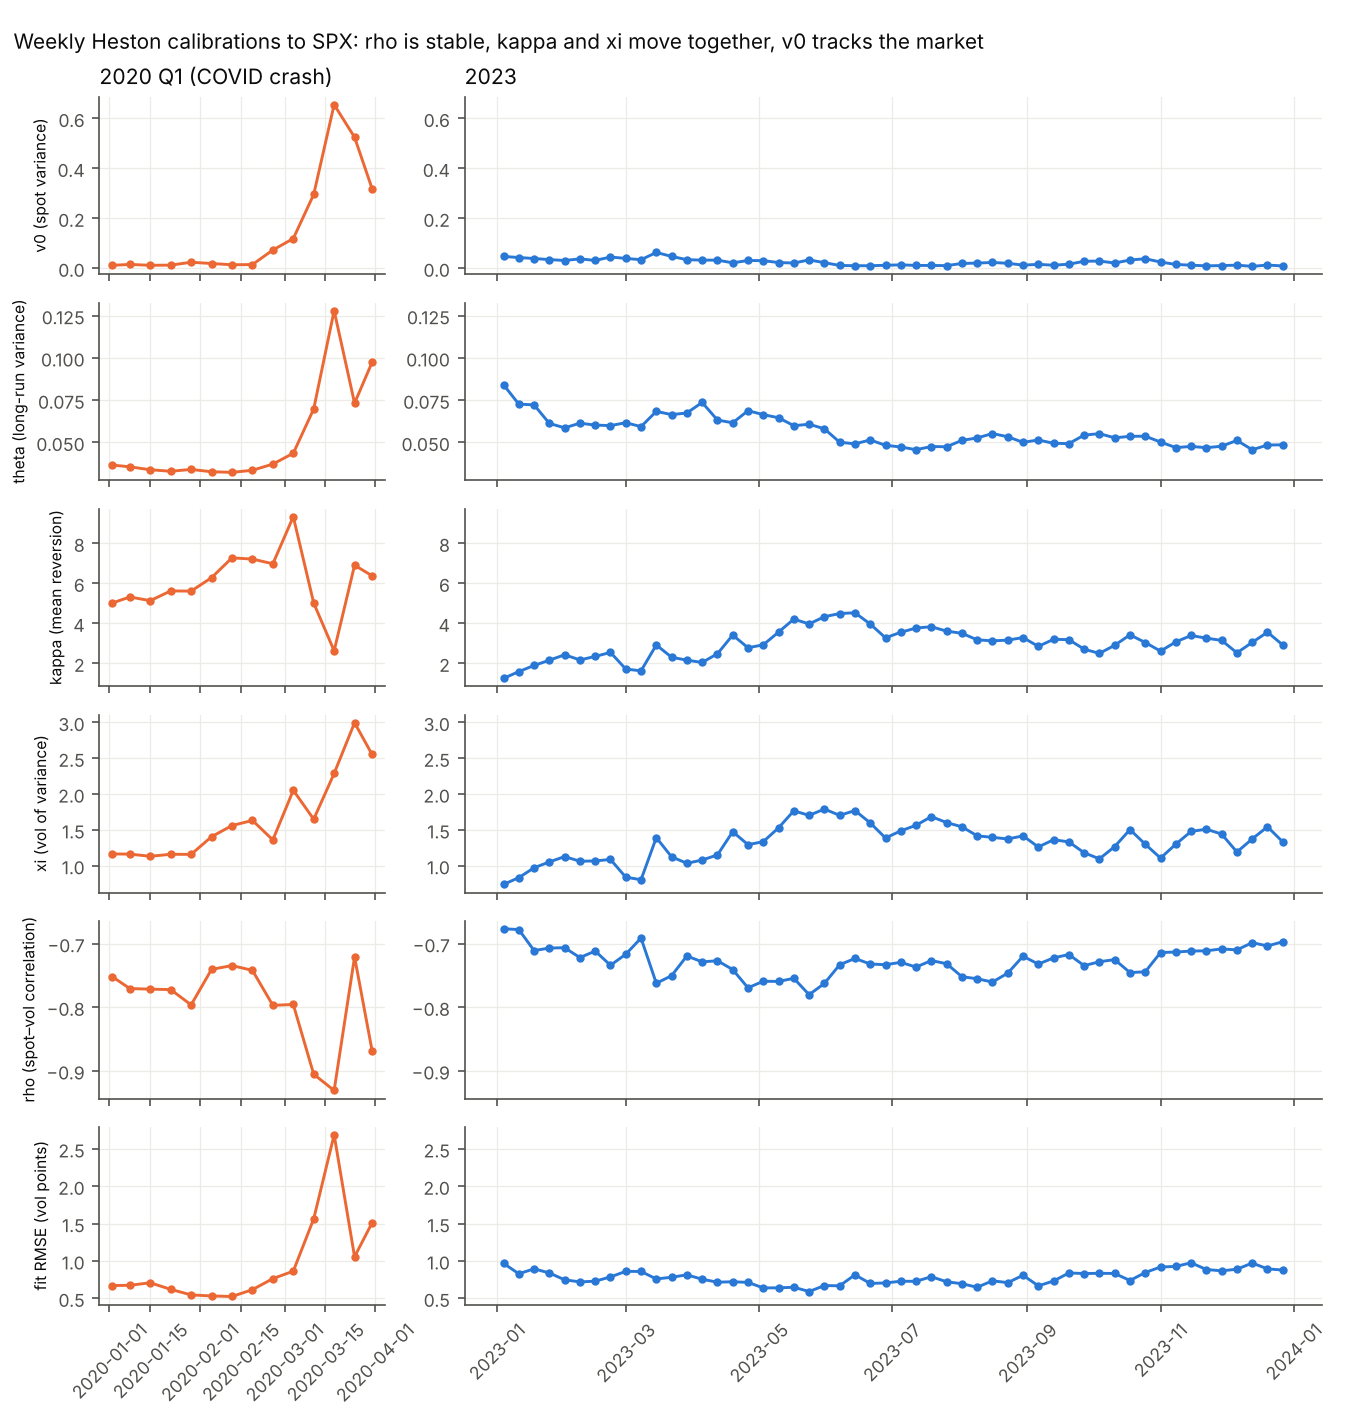
\includegraphics[width=0.74\textwidth]{spx_heston_param_timeseries.png}
\caption{Weekly Heston calibrations to SPX. $\rho$ is stable, $\kappa$ and $\xi$ move together, and $v_0$ tracks
short-dated implied vol. During the COVID crash every parameter and the fit error move sharply.}
\end{figure}

\begin{table}[H]
\caption{Heston parameter stability, 59 weekly fits in 2023}
\centering
\begin{tabular}{lrrr}
\toprule
\textbf{Parameter} & \textbf{Mean} & \textbf{Coefficient of variation} & \textbf{Corr.\ of weekly changes with $\Delta\kappa$}\\
\midrule
$\rho$ & $-0.73$ & 3\% & $-0.23$\\
$\theta$ & 0.056 & 15\% & $-0.27$\\
$\xi$ & 1.32 & 20\% & \textbf{0.96}\\
$\kappa$ & 2.99 & 25\% & 1\\
$v_0$ & 0.024 & 54\% & 0.05\\
Fit RMSE & 0.78\vp & 12\% & \\
\bottomrule
\end{tabular}
\end{table}

\begin{itemize}
\item \textbf{$\rho$ is the stable parameter.} The SPX skew is a persistent feature of the market.
\item \textbf{$\kappa$ and $\xi$ move together.} Their week-on-week changes have correlation 0.96, the ridge
predicted on synthetic data. The surface pins down a combination of the two, not each separately.
\item \textbf{$v_0$ is a state variable, not a parameter.} It should move, and it does: $\sqrt{v_0}$ has correlation
0.99 with 1-month at-the-money implied vol.
\item \textbf{The crisis breaks the fit.} From 2020-02-19 to 2020-03-18, $\sqrt{v_0}$ rises from 12\% to 81\%,
$\rho$ falls to $-0.93$ and the fit RMSE rises from below 1 to 2.7\vp.
\end{itemize}

\begin{caution}
\textbf{Practical consequence.} Any risk number that depends on $\kappa$ alone, such as sensitivity to the
long-run variance, is unreliable, and recalibrating daily injects noise into P\&L. Two remedies follow: fix
$\kappa$ and recalibrate the rest, or penalise changes from the previous day's parameters. A five-parameter
diffusion fits a calm surface well and a crisis surface badly, exactly when the model matters most.
\end{caution}

% ================================================================= 5 MODEL RISK
\section{Exotics and Model Risk}
\subsection{Products and their checks}
\textbf{Down-and-in barrier put.} The continuously monitored price has a closed form \citep{reiner1991}.
Daily monitoring is handled by the \citet{broadie1997} correction, which shifts the barrier away from spot
by $e^{-\beta\sigma\sqrt{\Delta t}}$ with $\beta = -\zeta(1/2)/\sqrt{2\pi}\approx 0.5826$. The shifted closed form
gives 4.92\% of spot for the 3-year 100/60 put; daily-monitored Monte Carlo gives $4.93 \pm 0.04$.

\textbf{Autocallable.} A 3-year note on SPX with notional 100 and quarterly observations. If the index is at or
above its initial level on an observation date, the note redeems at par plus an 8\% p.a.\ accrued coupon.
If it is never called and the index has ever closed below 60\% (daily knock-in), the holder receives
$100\,S_T/S_0$ when $S_T<S_0$; otherwise par. The note is priced by Monte Carlo and by two coupled PDEs
(``knocked in'' and ``not knocked in''), stepped once per business day. Under Black-Scholes the PDE gives 97.18
against $97.20 \pm 0.04$ by Monte Carlo; under local vol both give 96.63.

The present value is affine in the coupon, $PV(c) = A + cB$, so two pricings give the fair coupon
$c^\ast = (100 - A)/B$ at which the note is worth par.

\subsection{Same market, three models}
All three models are fitted to the 2023-01-18 SPX surface (spot 3945.1, implied $r=3.93\%$, $q=1.49\%$).
Black-Scholes uses the market at-the-money vol at the note's maturity, 20.65\%.

\begin{table}[H]
\caption{Autocallable and barrier put under three models fitted to the same surface}
\centering
\begin{tabular}{lrrrrr}
\toprule
\textbf{Model} & \textbf{Fair coupon} & \textbf{P(called, 1st date)} & \textbf{P(knock-in loss)} & \textbf{Exp.\ life (y)} & \textbf{DIP 100/60 (\% $S_0$)}\\
\midrule
Black-Scholes & 14.03\% & 50.3\% & 8.2\% & 0.96 & 4.93\\
Heston & 15.17\% & 63.8\% & 8.3\% & 0.73 & 9.32\\
Local vol & 15.95\% & 58.8\% & 8.9\% & 0.73 & 8.43\\
\bottomrule
\end{tabular}
\end{table}

\begin{figure}[htbp]
\centering
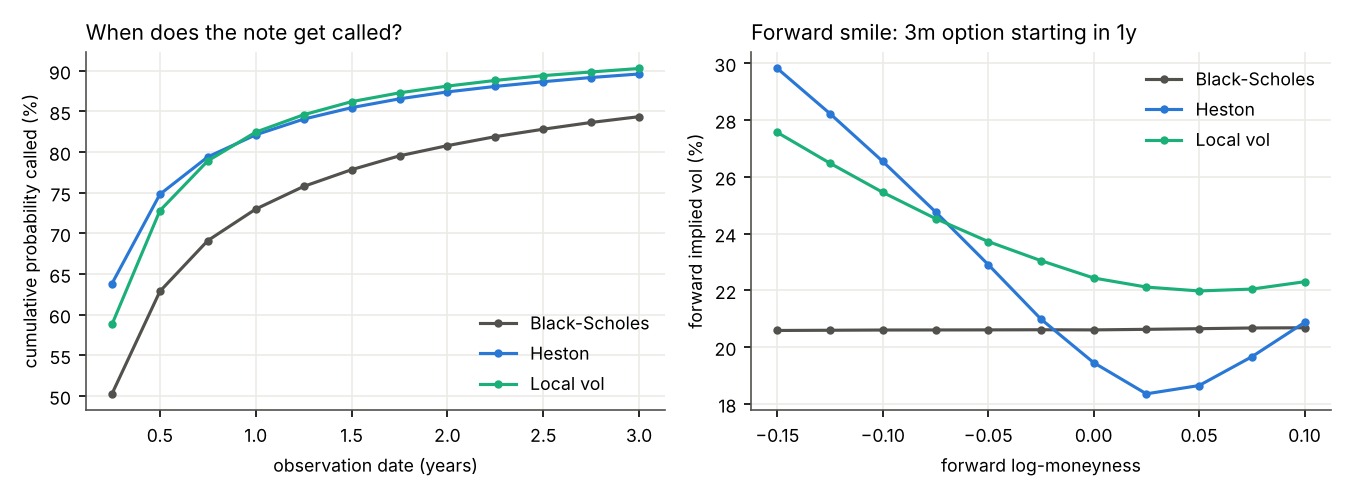
\includegraphics[width=\textwidth]{autocall_model_risk.png}
\caption{Left: cumulative probability that the note has been called by each observation date. Right: forward
smile, the implied vol of a 3-month option starting in one year, computed from each model's simulated paths.
Local vol's forward skew is flatter than Heston's.}
\end{figure}

\begin{callout}
\textbf{Economic interpretation.} Black-Scholes, with no skew, values the 60\% knock-in put at about half what the
skew-consistent models do, and so understates the coupon the issuer can afford. Heston and local vol both reproduce
the vanilla market, yet differ by 0.8 coupon points. The difference is the forward smile: local vol's skew flattens as
time passes, Heston's persists. A path-dependent payoff depends on those forward dynamics, which vanilla prices do not
pin down.
\end{callout}

The industry answer is stochastic local vol, which matches vanillas exactly and takes its forward-smile dynamics from a
stochastic component. That moves the model risk into a single mixing weight, which then becomes the parameter a desk
must reserve against.

% ================================================================= 6 HEDGING
\section{Greeks and the Sources of Hedging Error}
\subsection{Greeks without bumping}
Monte Carlo Greeks were implemented three ways. The pathwise estimator differentiates along each path,
$\Delta = \mathbb{E}[e^{-rT}\mathbf{1}\{S_T>K\}S_T/S_0]$, and fails for a digital option, whose payoff has zero
derivative almost everywhere. The likelihood-ratio estimator moves the derivative onto the density,
$\Delta = \mathbb{E}[e^{-rT}f(S_T)\,Z/(S_0\sigma\sqrt T)]$, and works for any payoff at the cost of higher variance. A
mixed estimator, likelihood ratio applied to the pathwise delta, gives gamma. All three match the closed forms within
three standard errors.

\subsection{The hedged P\&L identity}
For a short option that is delta-hedged and self-financed, the Black-Scholes PDE turns theta and financing into
$\tfrac12\Gamma S^2\sigma_{\text{imp}}^2\,dt$, so one day's P\&L is, to second order,
\begin{equation}
d\Pi \approx \underbrace{\tfrac12\Gamma S^2\left(\sigma_{\text{imp}}^2\,dt - \left(\tfrac{dS}{S}\right)^2\right)}_{\text{gamma/theta}}
\;-\; \underbrace{\mathcal{V}\,d\sigma_{\text{imp}}}_{\text{vega}}
\;-\; \underbrace{\left(\text{vanna}\cdot dS\,d\sigma_{\text{imp}} + \tfrac12\text{volga}\cdot d\sigma_{\text{imp}}^2\right)}_{\text{vanna/volga}}
\;+\;\varepsilon .
\end{equation}
The first term is the core of option trading: a short-gamma book earns when realised variance is below implied and loses
when it is above.

\subsection{Simulation: what discrete hedging costs}
In a Black-Scholes world with a 3-month at-the-money call and $\sigma=20\%$, the hedging error from rebalancing $N$ times
should follow \citet{kamal1999}:
\begin{equation}
\operatorname{sd}(\text{P\&L}) \approx \sqrt{\frac{\pi}{4}}\ \frac{\mathcal{V}\,\sigma}{\sqrt N}.
\end{equation}
With 63 daily rebalances the simulated standard deviation is 0.434 against 0.441 from the formula (per 100 notional).
Halving the error needs four times the trades. With 5 bp transaction costs, cost grows like $\sqrt N$ while hedging error
falls like $1/\sqrt N$, so there is an optimal frequency, near 252 rebalances here.

\begin{figure}[htbp]
\centering
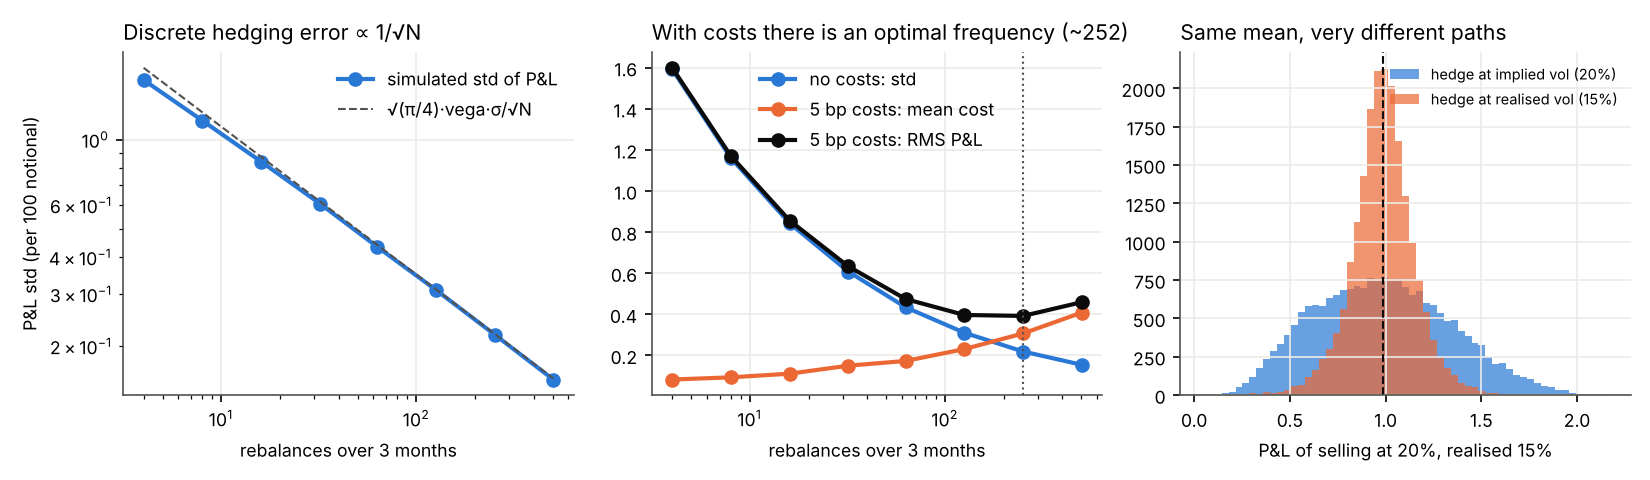
\includegraphics[width=\textwidth]{hedging_simulation.png}
\caption{Left: discrete-hedging error scales as $N^{-1/2}$ and matches Kamal--Derman. Centre: with 5 bp costs the RMS P\&L
has a minimum. Right: selling at 20\% implied when realised is 15\%; hedging with implied-vol deltas and with
realised-vol deltas gives the same mean (0.99) but very different dispersion (0.35 vs 0.16).}
\end{figure}

\subsection{Real SPX: short 1-month calls, hedged daily}
On the first trading day of each month, one 1-month at-the-money SPX call is sold at mid (strike nearest the implied
forward, expiry nearest 30 days), hedged daily in the index, and re-marked daily at market mid. Each day's P\&L is split
with the identity above using that day's implied vols.

\begin{table}[H]
\caption{Real SPX hedging backtest, index points per one call, no transaction costs}
\centering
\begin{tabular}{lrrrrrrrr}
\toprule
\textbf{Period} & \textbf{Trades} & \textbf{P\&L} & \textbf{Gamma/theta} & \textbf{Vega} & \textbf{Vanna/volga} & \textbf{Residual} & \textbf{Entry IV} & \textbf{Realised}\\
\midrule
2020 Q1 & 3 & $-127.8$ & $-96.4$ & $-65.5$ & 10.6 & 23.5 & 17.2\% & 36.3\%\\
2023 & 12 & $+31.8$ & $+73.6$ & $-75.6$ & 2.1 & 31.7 & 15.6\% & 12.1\%\\
\bottomrule
\end{tabular}
\end{table}

\begin{figure}[htbp]
\centering
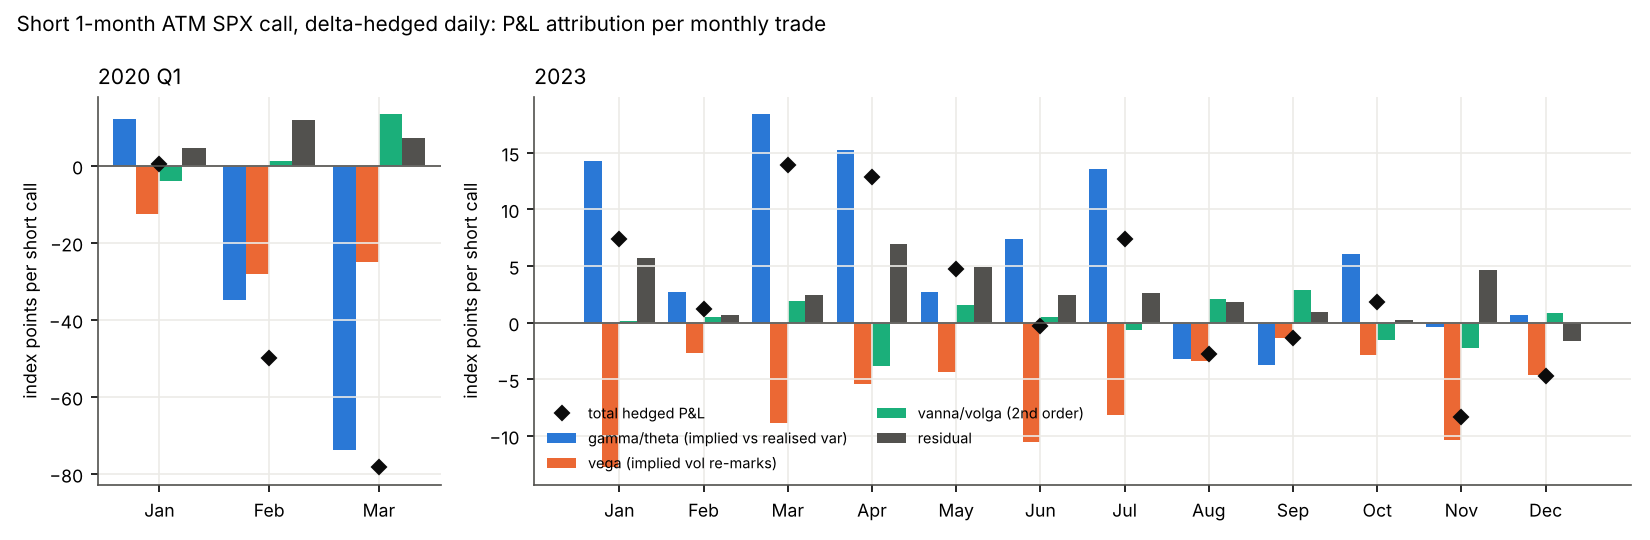
\includegraphics[width=\textwidth]{hedging_spx_attribution.png}
\caption{P\&L attribution per monthly trade. In 2023 gamma/theta (blue) is mostly positive, and most of it is given back
through vega (orange). In 2020 Q1 both lines are negative.}
\end{figure}

\begin{itemize}
\item \textbf{2023 is the variance risk premium at work.} Implied vol averaged 15.6\% against 12.1\% realised, and
gamma/theta earned $+73.6$ points over 12 trades. Most of it was given back through vega: in a rising market a fixed strike
slides down the skew, so its implied vol rises even when the smile itself does not move.
\item \textbf{2020 Q1 is the tail of selling volatility.} Realised vol of 36\% against 17\% implied cost 96.4 points in
gamma/theta in three trades.
\item \textbf{The Greeks explain most of the P\&L.} Gamma/theta and vega explain 86\% of the variance of daily hedged P\&L;
adding vanna and volga raises this to 91\%.
\end{itemize}

\begin{caution}
\textbf{Inference discipline.} Fifteen trades in two hand-picked windows cannot estimate the return of selling volatility,
and the March 2020 trade stops after eight days at the data cut-off. The backtest is evidence about \emph{where} hedged P\&L
comes from, not about how much a strategy would earn. The positive residual, concentrated on the largest down days, is still
unexplained; third-order spot terms and bid--ask noise in daily mids are the two candidates.
\end{caution}

% ================================================================= 7 LADDER
\section{Evidence Ladder}
The project supports five claims of different strength.
\begin{enumerate}
\item \textbf{Numerical correctness: strong.} Three engine types agree on every contract within discretisation or
statistical error, and each converges at its theoretical rate.
\item \textbf{Heston's short-end misfit is a model limitation: strong.} The calibrator recovers synthetic parameters to
$10^{-4}$, all starts agree, and the residuals have the structure diffusive stochastic vol predicts.
\item \textbf{$\kappa$--$\xi$ non-identifiability: strong.} Predicted on synthetic data before the SPX fits, then observed in
59 weekly fits (correlation 0.96).
\item \textbf{Model risk on path-dependent payoffs: strong for the mechanism, single-date for the size.} The forward-smile
explanation is shown directly; the 2-point coupon range is from one surface.
\item \textbf{P\&L attribution on real data: supportive.} The Greeks explain 91\% of daily P\&L variance, but over 15 trades
only.
\end{enumerate}

The contribution is therefore not a new model. It is a pricing library in which every number is checked by an
independent method, so that the differences that remain, between models and between hedge and reality, can be
attributed to their economic cause.

% ================================================================= 8 LIMITATIONS
\section{Limitations \& Next Tests}
\subsection{Current limitations}
\begin{itemize}
\item \textbf{Data:} end-of-day mids from a single vendor, without intraday synchronisation between the index and the
options; constant $r$ and $q$ per date when building local vol.
\item \textbf{Heston PDE:} there is no 2D (ADI) solver, so Heston prices are cross-checked by COS and Monte Carlo only.
\item \textbf{Models:} no jumps and no rough volatility, which the short-dated residuals call for.
\item \textbf{Model risk:} the coupon comparison uses one surface; its stability over time is untested.
\item \textbf{Trading frictions:} the real backtest sells at mid and hedges without cost.
\end{itemize}

\subsection{Highest-value next tests}
\begin{enumerate}
\item Stochastic local vol for the autocallable, with the mixing weight as an explicit model-risk parameter.
\item Andersen--Broadie dual upper bounds to bracket the Longstaff--Schwartz value from above.
\item A 2D Crank--Nicolson ADI solver for Heston, as a third independent engine.
\item A smile-adjusted (minimum-variance) delta in the backtest, to move the sticky-strike vega loss into the hedge.
\item Bid--ask and index-futures costs in the real backtest, and a full-revaluation P\&L explain to identify the residual.
\end{enumerate}

\section{Closing View}
The project starts with a narrow requirement: the same contract must get the same price from three unrelated methods.
Once that holds, the remaining disagreements become informative. Heston's 1-month error says that diffusion is not enough
at the short end. The $\kappa$--$\xi$ ridge says that a good fit can still leave parameters unidentified. The 2-point coupon
gap says that matching vanillas does not fix the price of path dependence. The hedging backtest says that the Black-Scholes
Greeks account for most, but not all, of what a hedged book earns.

Each of these is a statement about a model, not about the code. That is the purpose of the cross-validation.

% ================================================================= APPENDICES
\appendix
\section{Reproducibility Checklist}
\begin{itemize}
\item 70 unit tests (pytest) run in continuous integration on every push; they use synthetic inputs only and need no
market data.
\item Black-Scholes: textbook values, put--call parity, no-arbitrage bounds, Greeks against finite differences, and
Greeks satisfying the Black-Scholes PDE.
\item Heston COS: agreement with the \citet{lewis2001} integral by adaptive quadrature to $10^{-9}$, and the Black-Scholes
limit as $\xi\to0$ at rate $O(\xi^2)$.
\item PDE: convergence order on Europeans, American put against a binomial tree, barrier order with the grid aligned.
\item Monte Carlo: every estimator within three standard errors of the analytic value; Longstaff--Schwartz below the PDE
American value.
\item Calibration: implied forward recovered from synthetic chains; Heston parameter recovery with and without noise;
Dupire round trip on a synthetic surface to 0.03\vp.
\item Exotics: barrier closed form against PDE and Monte Carlo; autocallable PDE against Monte Carlo.
\item Hedging: Kamal--Derman scaling and the hedged P\&L identity on simulated paths.
\item Every formula in the code is derived in \texttt{docs/derivations/01}--\texttt{10}; each stage script regenerates its
tables and figures.
\end{itemize}

\bibliographystyle{plainnat}
\renewcommand{\bibfont}{\footnotesize}
\setlength{\bibsep}{2pt}
\renewcommand{\bibsection}{\needspace{12\baselineskip}\section*{References}\markboth{References}{}}
\bibliography{refs}

\end{document}
